\section{Systems Engineering}

Systems engineering is a branch of engineering used to help in the
design of complex systems. The general V\&V diagram for a systems life
cycle can be seen below.
\begin{figure}[H]
  \begin{center}
  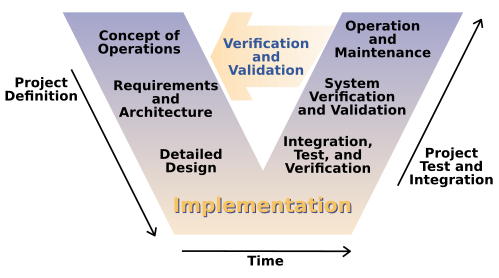
\includegraphics[height=70mm]{Figures/VandV}
  \end{center}
  \caption{Verification and Validation Diagram for a Systems
    Engineering Life Cycle \cite{vandv}}
\end{figure}
The left side of the V\&V diagram highlights all of the required
design while the right side details the build. 

\subsection{Interface Diagrams} 

Interface Diagrams (IDs) are important for many reasons. The biggest
reason that these diagrams are created and maintained is to create
visibility within each subsystem team in a systems engineering7
project. It is crucial that each member working on a project has a
general or even an expert understanding of each subsystem. During the
design process, it is important that each function of each subsystem’s
component is documented so that the current design selection is
recorded and so each of the member’s is familiar with each subsystem
and all of its functionalities. The following image is the ID for the
attitude control and maneuver electronics subsystem on the Gemini Spacecraft.  
\begin{figure}[H]
  \begin{center}
  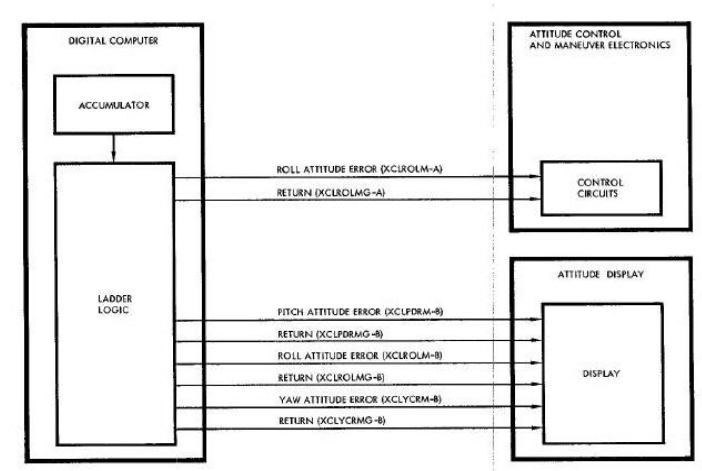
\includegraphics[height=70mm]{Figures/ACME_ID}
  \end{center}
  \caption{ACME Interface Diagram from the Gemini Spacecraft\cite{qp10}}
\end{figure}
This is an example of an interface diagram for a small subsystem of a
large systems engineering project. The spacecraft requires several
subsystems to work together in the design and fabrication
process. Each of these subsystems has their own ID as well. This is a
good example to introduce you to what these diagrams are. The left
side of the image is the digital computer  which has an accumulator
which flows to the ladder logic block. From the ladder logic flows
several functions into both the attitude control and maneuver
electronics and attitude display blocks. This ID is simple since there
are only four components with many functions, however, many
complicated systems can have extremely complex diagrams. The Figure
below is an example of an ID for an entire spacecraft with all of the 
subsystems included in the diagram.
\begin{figure}[H]
  \begin{center}
  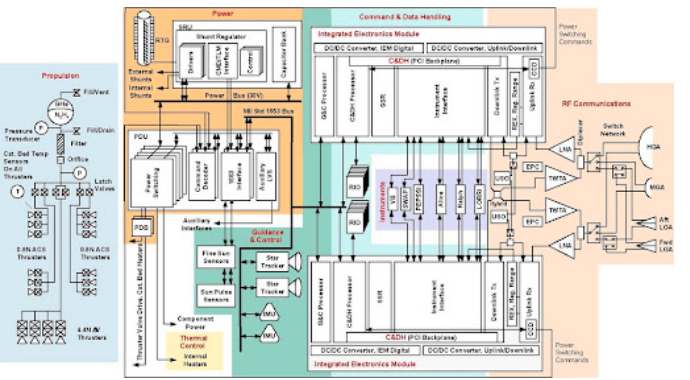
\includegraphics[height=70mm]{Figures/NewHorizons_ID}
  \end{center}
  \caption{New Horizons Interface Diagram\cite{qp11}}
\end{figure}
\subsection{Activity Diagrams}
Activity diagrams are similar to a flowchart.  It is a tool for
representing the sequence of Actions that describe the behavior of a
Block or other structural element. The sequence of execution is
defined using Control Flows. The Actions in an activity diagram can
contain Input and Output Pins which act as buffers for items that flow
from one action to another. Anything that can be produced, consumed,
or conveyed by the system is considered to be an item. Physical
materials, energy, power, data, and information are examples of items\cite{qp12}.

Activity diagrams are useful for engineering modeling.  It conveys
high-level functions and operations to the user. The main purpose of
an activity diagram is to draw the activity or action flow of a
system. Next, it is used to describe the sequence from one activity to
another. Finally, an activity diagram describes the parallel,
branched, and concurrent flow of the system \cite{qp13}.

Activity diagrams are important to the design process because they
maintain coherence throughout the project. If a system is composed of
multiple, intertwining subsystems, a person can simply follow the
activity diagrams to understand how each component and subsystem
interacts with one another. Activity diagrams also describe the data
flow of a system and when or where that data is created, converted or
used. Overall, activity diagrams are the roadmap of a system and
describe the intricacies of how it operates.  

As stated previously, activity diagrams denote how components and
subsystems interact with each other. This is accomplished through the
use of swimlanes which keep separate the individual activities and
object flows of a component or subsystem. Swimlanes are the boxes
which contain activities, however control and object flows can
traverse swimlanes. Activities which have inputs and outputs will also
have a pin attached to them. This small rectangular box denotes when
matter, energy or data flow is created or destroyed.  

The main purpose of activity diagrams is to show the control flow of
the system. This control flow refers to the execution path of an
activity. Control flow is indicated by control nodes for which there
are seven different kinds. Each control node is described in the table below.
\begin{table}[H]
  \begin{center}
    \begin{tabular}{c|p{7cm}|c}
      \hline
      Control Node & Description & Appearance \\
      \hline
      \hline
      Initial Node & The beginning of an activity sequence & Black
      circle \\
      \hline
      Activity Final Node & The end of an activity sequence & Black
      circle within a circle \\
      \hline
      Flow Final Node & The end of one branch of an activity sequence,
      but not the entire activity diagram. & Circle with an 'X' in it
      \\
      \hline
      Decision Node & The splitting point of an activity flow based on
      the outcome of a boolean operator such as ‘isCommandValid
      ==True’. One flow in comes in, while two flows come out as
      branching paths. & Diamond \\
      \hline
      Merge Node & The merging point of two activity paths. Two flows
      come in, while one flow comes out. & Diamond \\
      \hline
      Fork Node & The distribution of an activity flow into multiple
      pathways. When one object or control token comes in, it is
      duplicated into multiple paths. & Black bar \\
      \hline
      Join Node & The joining point of multiple synchronized
      concurrent flows. Two concurrent flows come in, while one flow
      comes out. & Black bar \\
      \hline
      \hline
    \end{tabular}
  \end{center}
\end{table}
